%\documentclass[a4paper, 12pt]{scrreprt}

\documentclass[a4paper, 12pt]{scrartcl}
%usepackage[german]{babel}
\usepackage{microtype}
%\usepackage{amsmath}
%usepackage{color}
\usepackage[utf8]{inputenc}
\usepackage[T1]{fontenc}
\usepackage{wrapfig}
\usepackage{lipsum}% Dummy-Text
\usepackage{multicol}
\usepackage{alltt}
%%%%%%%%%%%%bis hierhin alle nötigen userpackage
\usepackage{tabularx}
\usepackage[utf8]{inputenc}
\usepackage{amsmath}
\usepackage{amsfonts}
\usepackage{amssymb}
\usepackage{graphicx}
\usepackage{longtable}
\usepackage{booktabs}
\usepackage{tabularx}
\usepackage{siunitx}

%\usepackage{wrapfig}
\usepackage[ngerman]{babel}
\usepackage[left=25mm,top=25mm,right=25mm,bottom=25mm]{geometry}
%\usepackage{floatrow}
\setlength{\parindent}{0em}
\usepackage[font=footnotesize,labelfont=bf]{caption}
\numberwithin{figure}{section}
\numberwithin{table}{section}
\usepackage{subcaption}
\usepackage{float}
\usepackage{url}
\usepackage{fancyhdr}
\usepackage{array}
\usepackage{geometry}
%\usepackage[nottoc,numbib]{tocbibind}
\usepackage[pdfpagelabels=true]{hyperref}
\usepackage[font=footnotesize,labelfont=bf]{caption}
\usepackage[T1]{fontenc}
\usepackage {palatino}
%\usepackage[numbers,super]{natbib}
%\usepackage{textcomp}
\usepackage[version=4]{mhchem}

\usepackage{hyperref}
\begin{document}

\section{Auswertung}

Es wurde die Veränderung des optischen Drehwinkels $\alpha$ über die Zeit bei unterschiedlichen Temperaturen gemessen. Diese Werte wurden in Abbildung ref{at} dargestellt


\begin{figure}[h]
	\centering	
	\begin{minipage}{1\textwidth}
	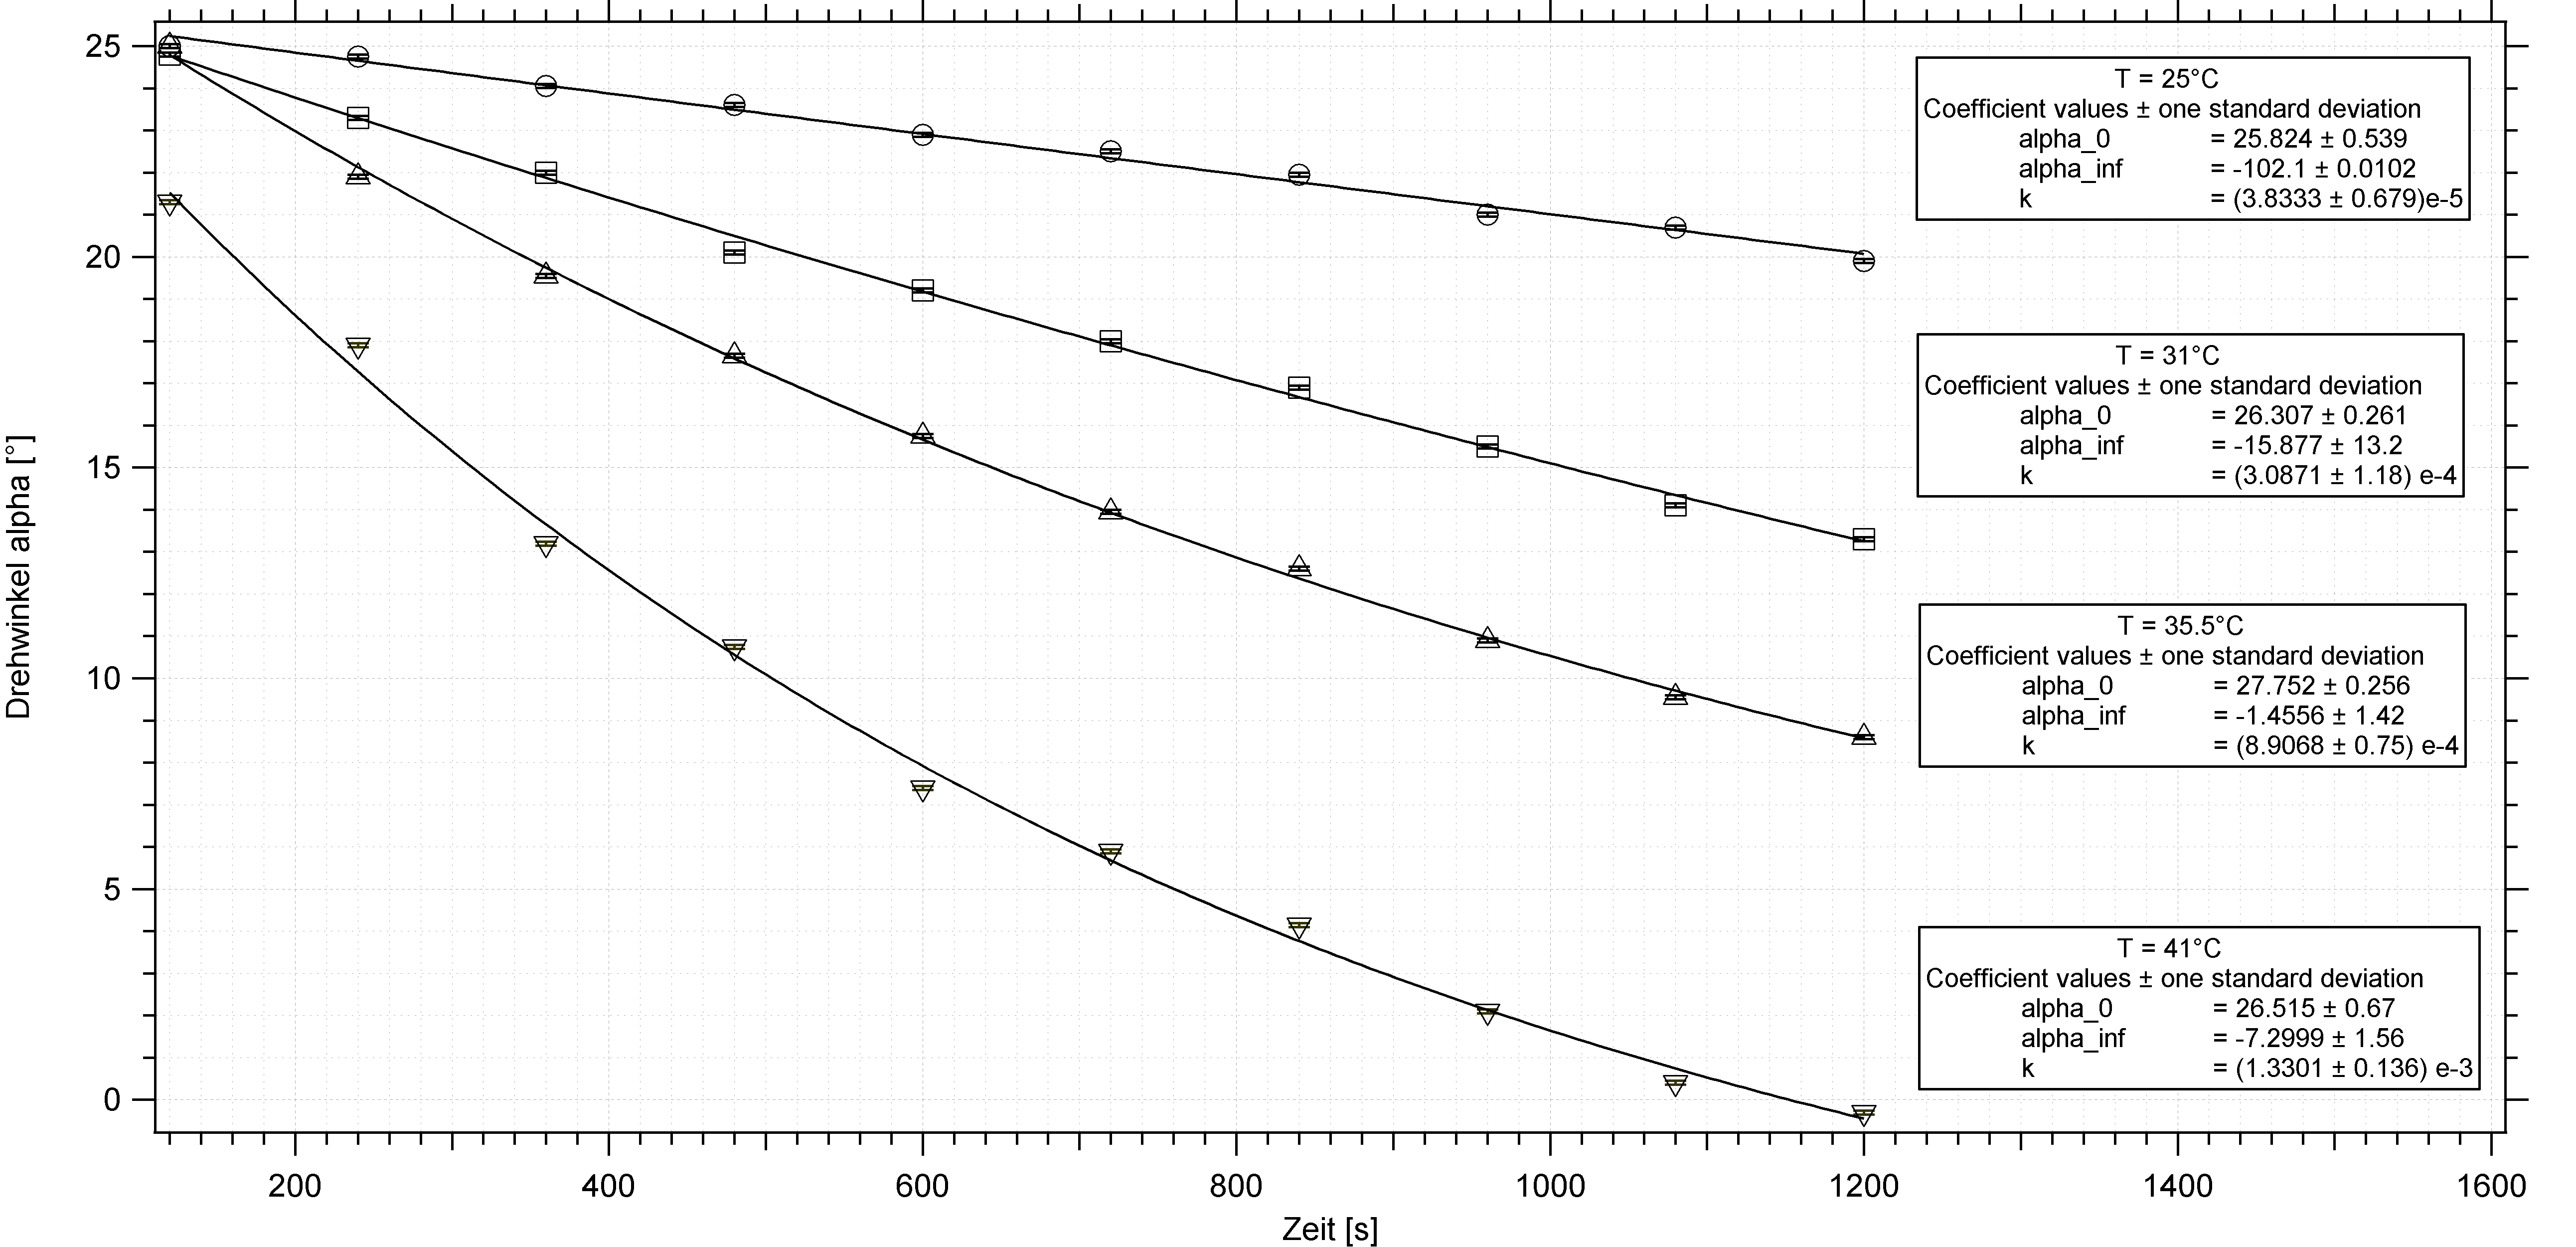
\includegraphics[width=\columnwidth]{Bilder/Graph1.png}
	\end{minipage}
		\caption{Auftragung des optischen Drehwinkels gegen die Zeit bei 25°C, 31°C, 35.5°C, 41°C zur Bestimmung von$\alpha_0$, $\alpha_\infty$ sowie von k bei der Hydrolyse von Saccharose ($25 Gew.\%$) mit $3-N$ HCL. Die Auswertung erfolgte mit Igor Pro 6.37 und einer, vom Assistenten zur Verfügung gestellten, Anpassungsfunktion.}
	\label{at}
\end{figure}
%%%%%%%%%%%%%%%%%%%%%%%

\begin{table}[H]

 
 
 \caption{Zusammenfassung der Reaktionskonstanten der Anpassung mit Gleichung XXX in Relation zur Temperatur.}
\begin{tabular}{L{0.5\linewidth}L{0.5\linewidth}}
Temperatur $[°C]$ & Reaktionskonstante $[???]$  \\
\hline \addlinespace[1ex] 
$25$ & $3.83\cdot 10^{-5}$ \\
$31$ & $3.09\cdot 10^{-4}$ \\
$35.5$ & $8.91\cdot 10^{-4}$ \\
$41$ & $1.33\cdot 10^{-3}$ \\
 \end{tabular}
 \label{tab1}
 \end{table}
\begin{equation}
k_T = k_\infty \cdot e^{\frac{E_a}{RT}}
\end{equation}
\begin{equation}
ln(k_T) = ln(k_\infty) + \frac{E_a}{RT}
\end{equation}
\begin{equation}
ln(k_T) = \frac{E_a}{R} \cdot \frac{1}{T} + ln(k_\infty) 
\end{equation}
Anschießend wurden der Natürliche Logarithmus von $k_T$ gegen $\frac{1}{T}$ gemäß der Arrhenius-Gleichung REF aufgetragen. Durch eine lineare Regression konnten somit $E_a$ und $k_\infty$ bestimmt werden. Dies ist in Abbildung \ref{ln} dargestellt.
\begin{figure}[h]
	\centering	
	\begin{minipage}{1\textwidth}
	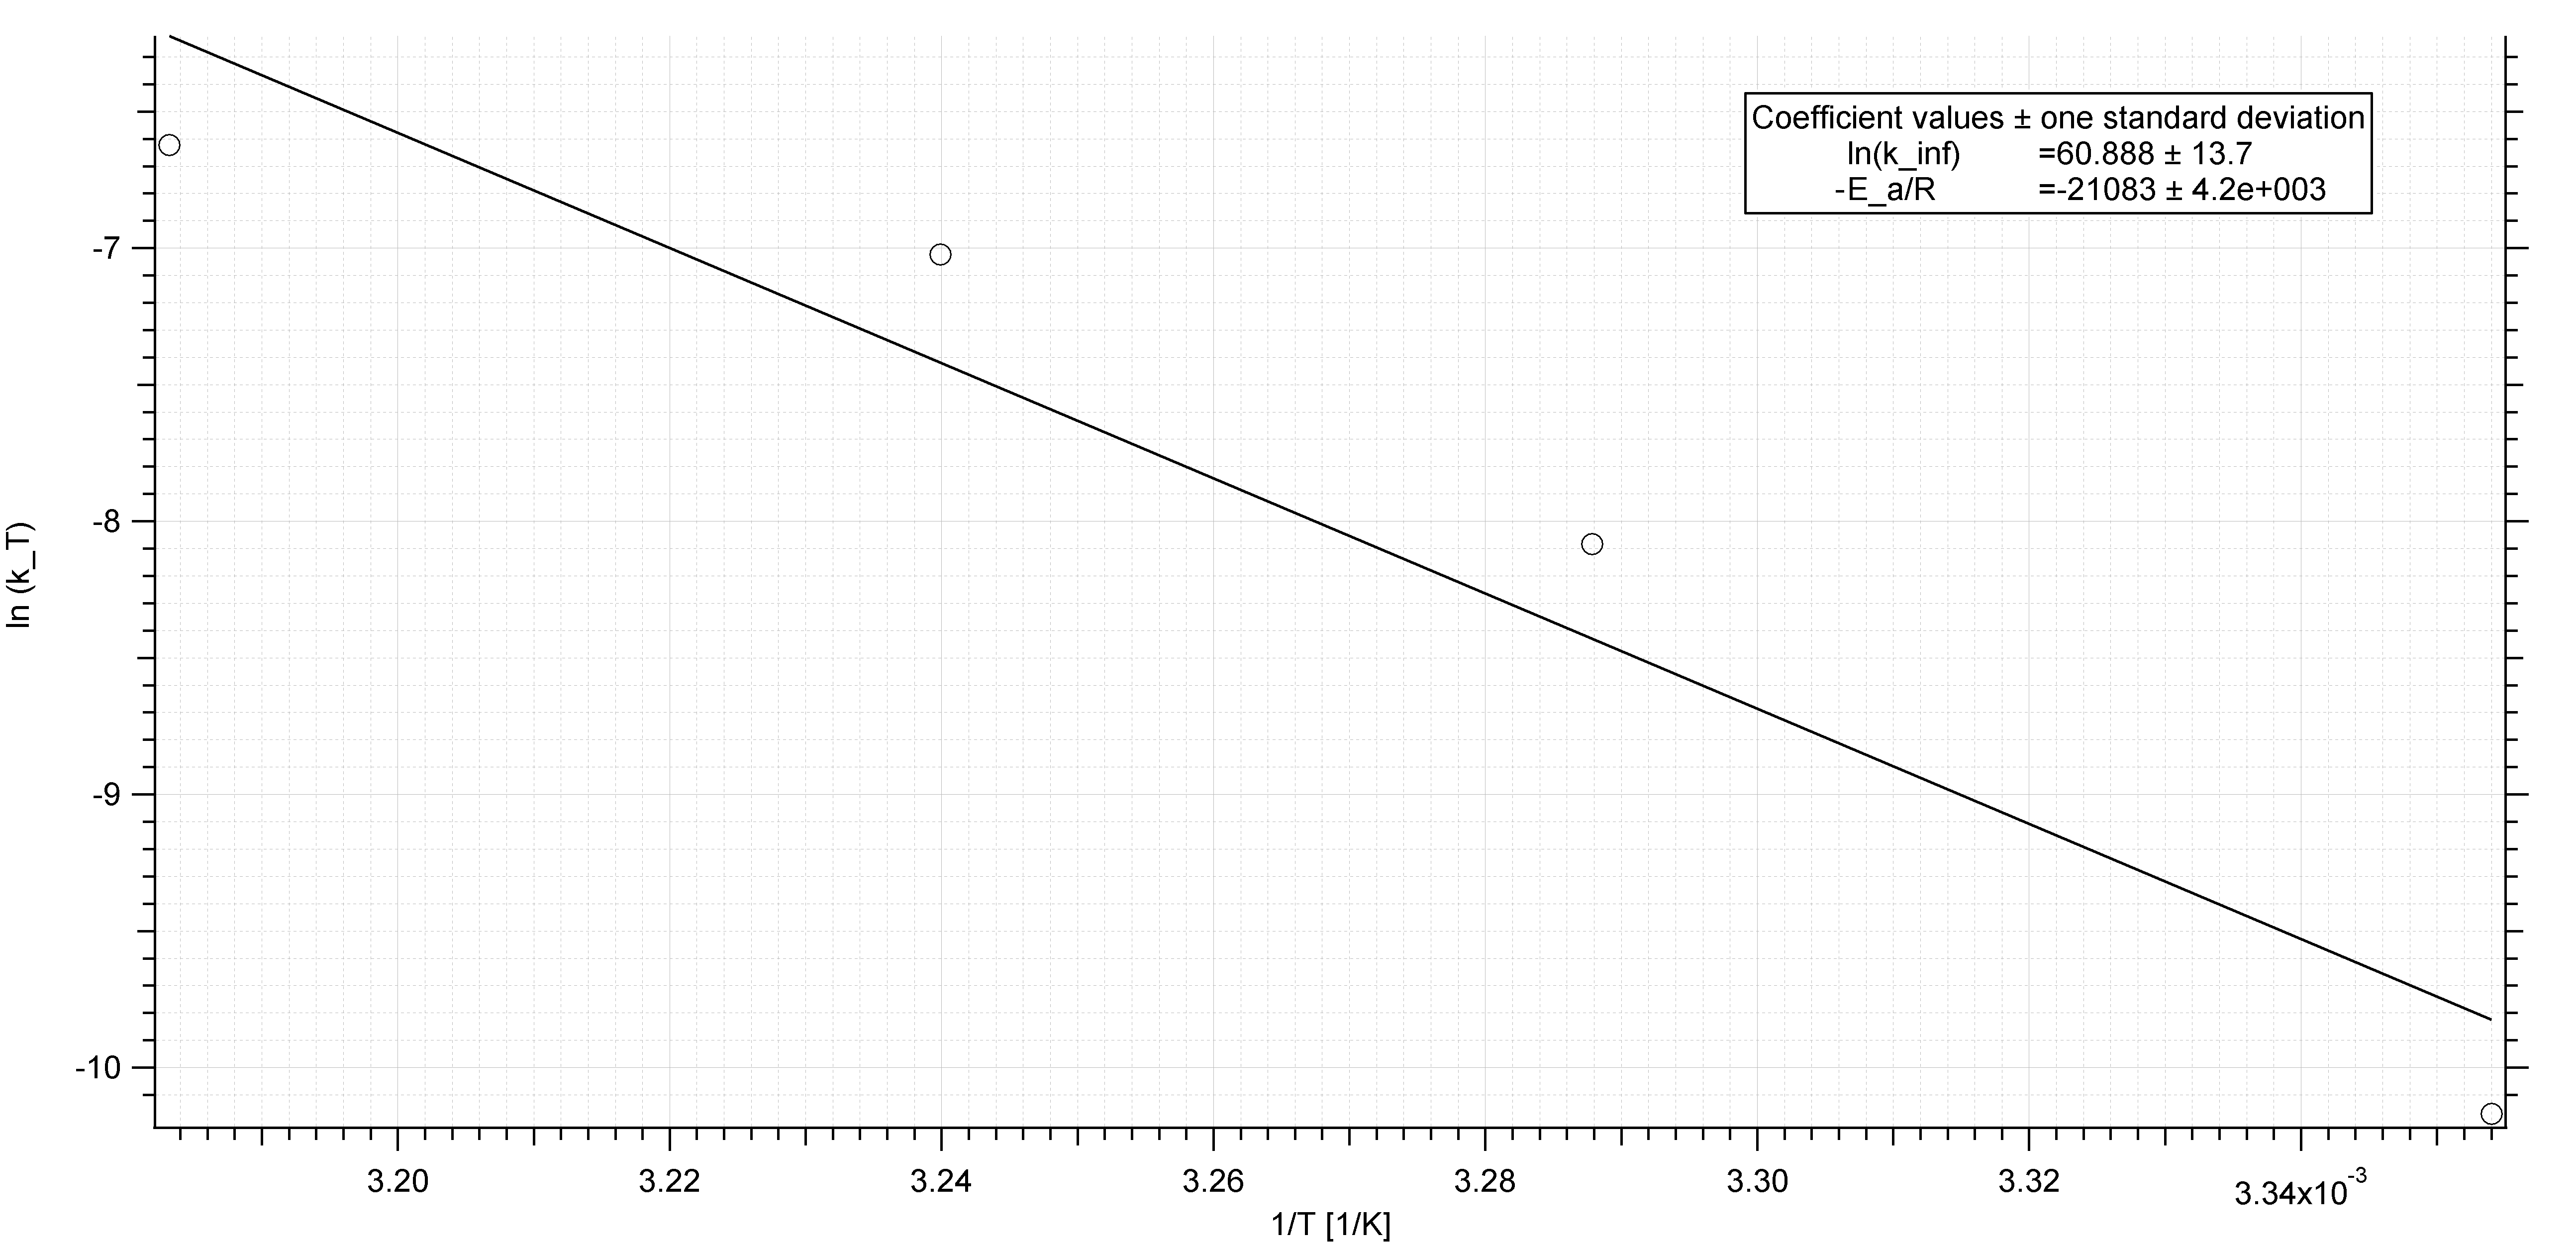
\includegraphics[width=\columnwidth]{Bilder/Graph2.png}
	\end{minipage}	
	\caption{Auftragung von $k_T$ über $\frac{1}{T}$ zur Bestimmung von $E_a$ und $k_\infty$ mittels einer linearen Regression der logarithmierten Arrhenius-Gleichung. Die Auswertung erfolgte mit Igor Pro 6.37}
	\label{ln}
\end{figure}

\begin{table}[H]

 
 
 \caption{Zusammenfassung der Ergebnisse der lineraren Regression der logarithmierten Arrhenius-Gleichung in Gegenüberstellung zur Literatur.}
\begin{tabular}{L{0.25\linewidth}L{0.25\linewidth}L{0.25\linewidth}R{0.25\linewidth}}
Konstante & Einheit & Messwert & Literatur cite{}\\
\hline \addlinespace[1ex] 
$ k_\infty$ & $ \frac{1}{s} $ & $ 2.77\cdot 10^{26}$  & \\
$ E_a $ & $ \frac{kJ}{mol} $ & $175 \pm 35$ & \\


 \end{tabular}
 \label{tab2}
 \end{table}

\end{document}
